\documentclass[tikz,border=8pt]{standalone}
\usepackage{tikz}
\usetikzlibrary{positioning,fit,backgrounds,calc,arrows.meta}
\usepackage{xcolor}

\definecolor{ugmblue}{HTML}{194168}
\definecolor{degreen}{RGB}{76,175,80}
\definecolor{dered}{RGB}{229,115,115}

\begin{document}
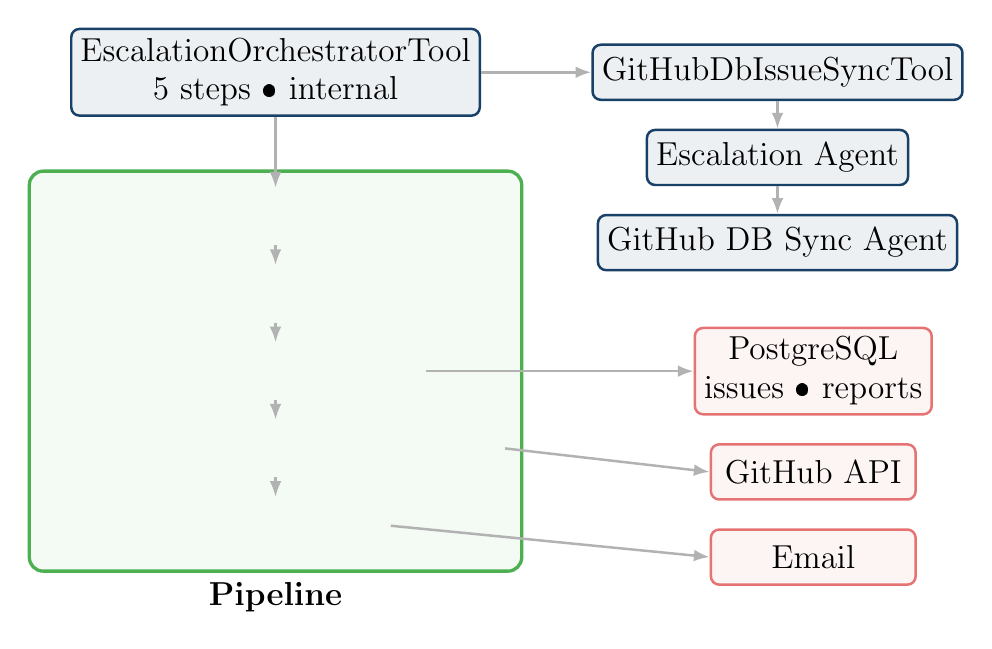
\begin{tikzpicture}[
    node distance=0.4cm and 0.5cm,
    box/.style={rectangle, rounded corners=3pt, draw=#1, fill=#1!8,
                minimum width=2.6cm, minimum height=0.7cm, align=center,
                line width=0.9pt, font=\large},
    group/.style={rectangle, rounded corners=5pt, draw=#1, fill=#1!6,
                  inner sep=6pt, line width=1.2pt},
    arr/.style={-{Latex[length=2mm]}, line width=0.9pt, draw=gray!60},
    lbl/.style={font=\large\bfseries}
]

% Top row: orchestrator + agents (left to right)
\node[box=ugmblue] (orch) {EscalationOrchestratorTool\\5 steps \textbullet{} internal};
\node[box=ugmblue, right=1.4cm of orch] (sync) {GitHubDbIssueSyncTool};
\node[box=ugmblue, below=0.35cm of sync] (sub1) {Escalation Agent};
\node[box=ugmblue, below=0.35cm of sub1] (sub2) {GitHub DB Sync Agent};

% Pipeline steps (left, vertical)
\node[box=degreen, below=0.9cm of orch, xshift=0cm] (s1) {1 \textbullet{} Fetch issues};
\node[box=degreen, below=0.25cm of s1] (s2) {2 \textbullet{} Detect recurring};
\node[box=degreen, below=0.25cm of s2] (s3) {3 \textbullet{} Lookup GitHub};
\node[box=degreen, below=0.25cm of s3] (s4) {4 \textbullet{} Comment / Create / Close};
\node[box=degreen, below=0.25cm of s4] (s5) {5 \textbullet{} Send email};
\node[group=degreen, fit=(s1)(s2)(s3)(s4)(s5),
      label={[lbl]below:Pipeline}] (pipe) {};

% Data sources (right column)
\node[box=dered, right=3.4cm of s3] (db) {PostgreSQL\\issues \textbullet{} reports};
\node[box=dered, below=0.35cm of db] (gh) {GitHub API};
\node[box=dered, below=0.35cm of gh] (em) {Email};

\draw[arr] (orch.south) -- (s1.north);
\draw[arr] (s1.south) -- (s2.north);
\draw[arr] (s2.south) -- (s3.north);
\draw[arr] (s3.south) -- (s4.north);
\draw[arr] (s4.south) -- (s5.north);
\draw[arr] (s3.east) -- (db.west);
\draw[arr] (s4.east) -- (gh.west);
\draw[arr] (s5.east) -- (em.west);
\draw[arr] (orch.east) -- (sync.west);
\draw[arr] (sync.south) -- (sub1.north);
\draw[arr] (sub1.south) -- (sub2.north);

\end{tikzpicture}
\end{document}
